\documentclass{beamer}

\usepackage{xcolor}
\usepackage{graphicx}
\usepackage{varwidth}
% \usepackage{caption}

\usepackage{subcaption}
\usepackage{media9}
\usepackage{multimedia}

\usepackage{amsfonts,amsmath,amssymb}

\usepackage{pgfplots}
\usepackage{tikz}
\usepackage{filecontents}
\usepackage{lmodern}

\usetikzlibrary{hobby}
\usetikzlibrary{decorations.shapes}
\usetikzlibrary{shadows.blur}

\definecolor{NvidiaGreen}{RGB}{118, 185, 0}

\usetheme{Madrid}
\setbeamertemplate{navigation symbols}{}

% Set the colors for various Beamer elements
\setbeamercolor{title}{fg=black, bg=NvidiaGreen} 
\setbeamercolor{frametitle}{fg=black, bg=NvidiaGreen} 
\setbeamercolor{item}{fg=black, bg=NvidiaGreen} 
\setbeamercolor{section in toc}{fg=black, bg=NvidiaGreen}
\setbeamercolor{author}{fg=white, 
        % bg=NvidiaGreen
    }
\setbeamercolor{date}{fg=white, 
        % bg=NvidiaGreen
    }

% Set the background to white for a clean presentation
\setbeamercolor{background canvas}{bg=white}

% #########################################################################################
% #########################################################################################
% Title
% #########################################################################################
% #########################################################################################

\begin{document}
{
\setbeamertemplate{background} 
{
    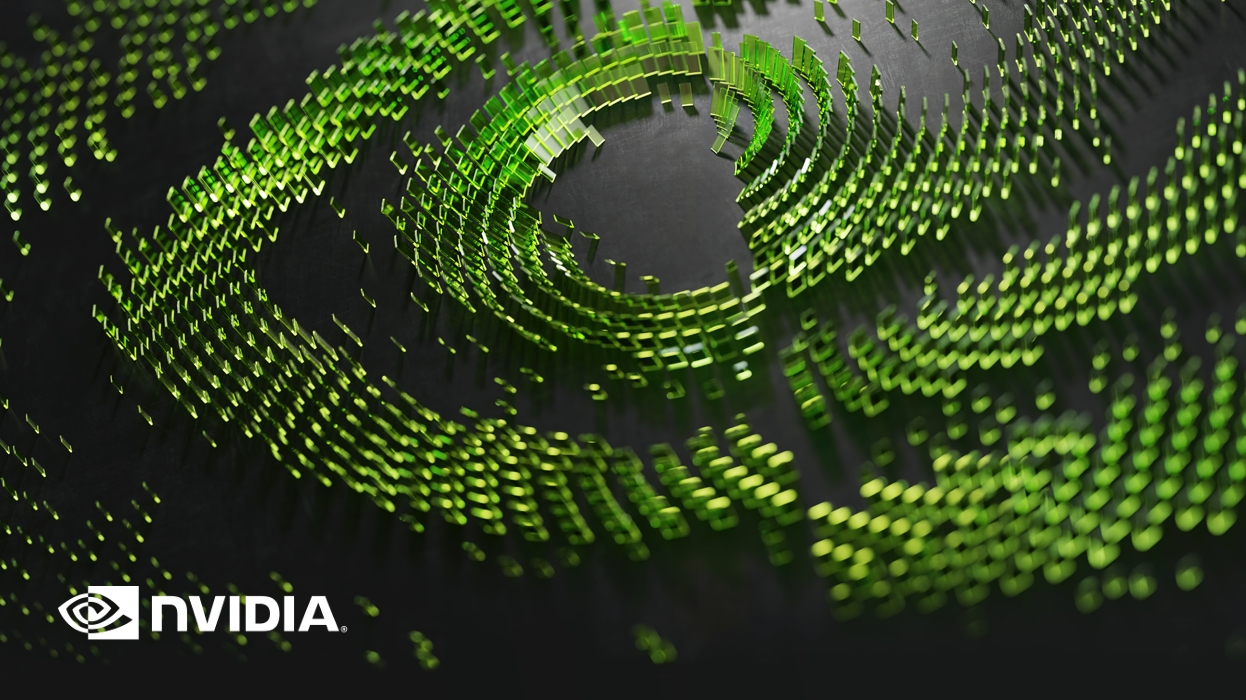
\includegraphics[width=\paperwidth,height=\paperheight]{images/Screenshot_9-12-2024_212019_.jpeg}
}
\title{\textbf{Towards Embodied Intelligence}}
\author[]{\textbf{Renan Monteiro Barbosa}}
% \date{\today}
\date[]{\textbf{2025}}
\maketitle
}

% #########################################################################################
% #########################################################################################
% Slide 1 - Intro
% #########################################################################################
% #########################################################################################

\section{LeatherBack Project}
\begin{frame}
\frametitle{\textbf{LeatherBack Project} }
The development of computer vision models has progressed rapidly, from YOLO’s fast and efficient real-time object detection to the powerful and flexible Vision Transformers. Both models represent milestones in the field, with YOLO excelling in speed and ViT pushing the boundaries of performance in image recognition. The future of computer vision is bright, with ongoing research promising even more breakthroughs.
\end{frame}

% #########################################################################################
% #########################################################################################
% Slide 2 - Test1 - Draw path on grid
% #########################################################################################
% #########################################################################################

\section{Test1 - Draw path on grid}
\begin{frame}
\frametitle{\textbf{Test1 - Draw path on grid} }

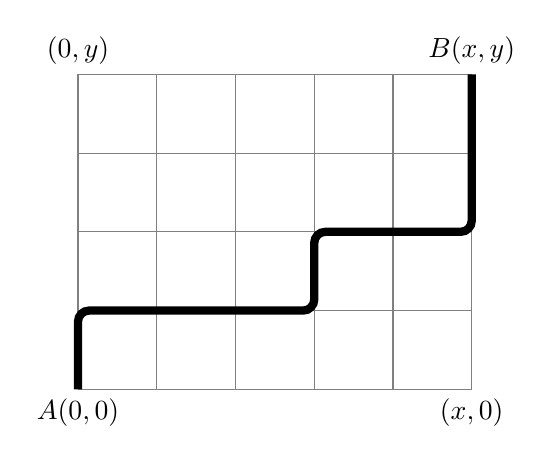
\begin{tikzpicture}
    \draw[step=1cm, color=gray] (0, 0) grid (5, 4);
   
   \foreach \coord/\label [count=\xi] in {
       {0,0}/{$A(0, 0)$},
       {5,4}/{$B(x, y)$},
       {5,0}/{$(x, 0)$},
       {0,4}/{$(0, y)$}
   }{
       \pgfmathsetmacro\anch{mod(\xi,2) ? "north" : "south"}
       \node[anchor=\anch] at (\coord) {\label};
   }
   
   \draw[line width=3pt, rounded corners] (0,0) -- (0,1) -- (3,1) -- (3,2) -- (5,2) -- (5,4);
   
\end{tikzpicture}

\end{frame}

% #########################################################################################
% #########################################################################################
% Slide 3 - Test2 - Grid numbering and repoeating structures
% #########################################################################################
% #########################################################################################

\section{Test2 - Grid numbering and repoeating structures}
\begin{frame}
\frametitle{\textbf{Test2 - Grid numbering and repoeating structures} }

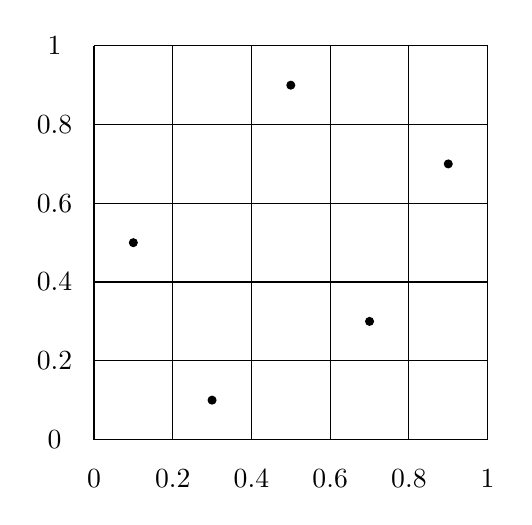
\begin{tikzpicture}
    \draw[step=1cm,black,thin] (0,0) grid (5,5);
    \foreach \xtick in {0,...,5} {\pgfmathsetmacro\result{\xtick * .2} \node at (\xtick,-0.5) {\pgfmathprintnumber{\result}}; }
    \foreach \ytick in {0,...,5} {\pgfmathsetmacro\result{\ytick * .2} \node at (-.5,\ytick) {\pgfmathprintnumber{\result}}; }
    \foreach \x/\y in {.5/2.5, 1.5/.5, 2.5/4.5, 3.5/1.5, 4.5/3.5}{\draw [fill=black, thin] (\x,\y) circle [radius=0.05];}
\end{tikzpicture}

\end{frame}

% #########################################################################################
% #########################################################################################
% Slide 4 - Test3 - Hypothesis Space representation Reference Image
% #########################################################################################
% #########################################################################################

\section{Hypothesis Space representation Reference Image}
\begin{frame}
\frametitle{\textbf{Test3 - Hypothesis Space representation Reference Image}}
\centering
\begin{minipage}{1\textwidth}
    \centering
    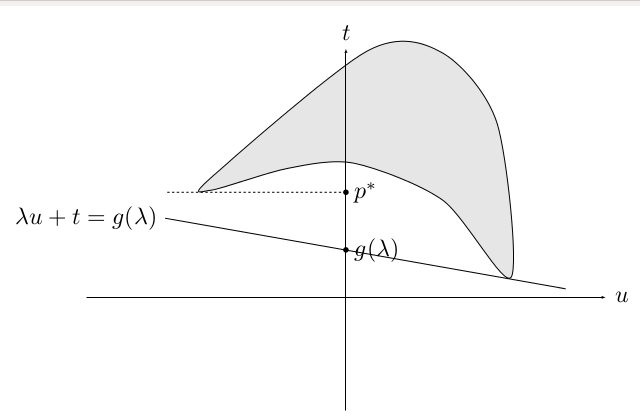
\includegraphics[width=0.8\textwidth]{images/reference_image.png} % Replace with your image file
    \captionof{figure}{reference image.}
\end{minipage}
\end{frame}

% #########################################################################################
% #########################################################################################
% Slide 5 - Test3 - Hypothesis Space representation
% #########################################################################################
% #########################################################################################

\section{Test3 - Hypothesis Space representation}
\begin{frame}
\frametitle{\textbf{Test3 - Hypothesis Space representation} }

% for some reason this does not fit on the Slide

Using the makebox method

\makebox[\textwidth][c]{ %
    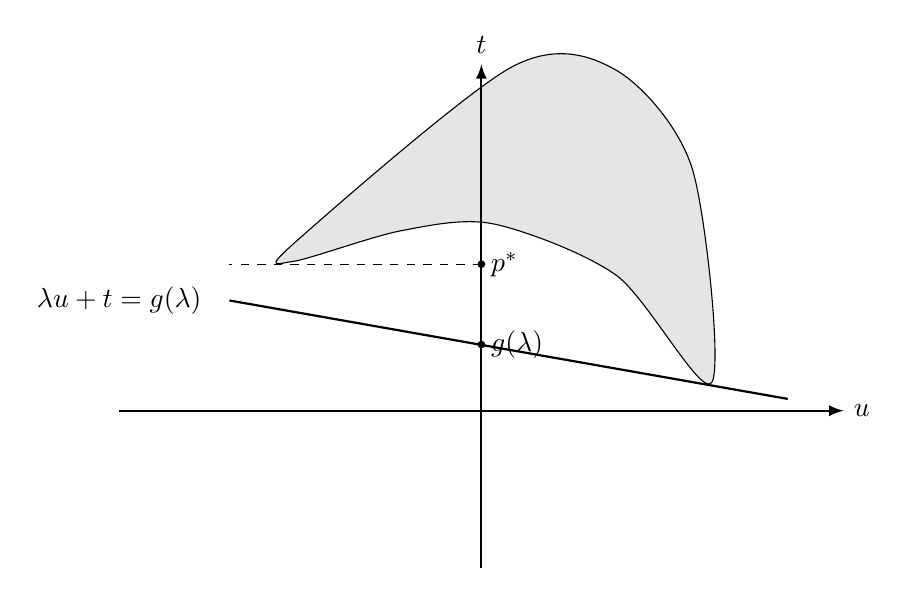
\begin{tikzpicture}[scale=0.4]
        \draw [fill=gray!20] plot [mark=none, smooth cycle] coordinates {(-5.97,4.742) (-2.554,5.713) (0.393,5.929) (4.295,4.291) (7.312,0.891) (6.7,7.668) (4.264,10.821) (0.948,10.904) (-5.973,5.294)};
        \draw [thick,-latex] (-11.5,0) -- (11.5,0) node [right,scale=1] {$u$};
        \draw [thick,-latex] (0,-5) -- (0,11) node [above,scale=1] {$t$};
        \draw [dashed] (0,4.65) -- + (-8,0);
        \draw [thick] (-8,3.5) -- + (-10:18);
        \node [scale=1] at (-11.5,3.5) {$\lambda u+t=g(\lambda)$};
        \coordinate (g) at (0,2.1);
        \fill (g) circle (3.5pt) node [right,scale=1] {$g(\lambda)$};
        \coordinate (p) at (0,4.65);
        \fill (p) circle (3.5pt) node [right,scale=1] {$p^{*}$};
    \end{tikzpicture} %
}

\end{frame}

% #########################################################################################
% #########################################################################################
% Slide 6 - Test3 - Hypothesis Space representation using hbox
% #########################################################################################
% #########################################################################################

\section{Test3 - Hypothesis Space representation}
\begin{frame}
\frametitle{\textbf{Test3 - Hypothesis Space representation} }

% for some reason this does not fit on the Slide

Using the hbox method

\setbox1=\hbox{%
    % \begin{tikzpicture}[use Hobby shortcut,closed=true]
    \begin{tikzpicture}[scale=0.3]
        \draw [fill=gray!20] plot [mark=none, smooth cycle] coordinates {(-5.97,4.742) (-2.554,5.713) (0.393,5.929) (4.295,4.291) (7.312,0.891) (6.7,7.668) (4.264,10.821) (0.948,10.904) (-5.973,5.294)};
        \draw [thick,-latex] (-11.5,0) -- (11.5,0) node [right,scale=1] {$u$};
        \draw [thick,-latex] (0,-5) -- (0,11) node [above,scale=1] {$t$};
        \draw [dashed] (0,4.65) -- + (-8,0);
        \draw [thick] (-8,3.5) -- + (-10:18);
        \node [scale=1] at (-11.5,3.5) {$\lambda u+t=g(\lambda)$};
        \coordinate (g) at (0,2.1);
        \fill (g) circle (3.5pt) node [right,scale=1] {$g(\lambda)$};
        \coordinate (p) at (0,4.65);
        \fill (p) circle (3.5pt) node [right,scale=1] {$p^{*}$};
    \end{tikzpicture} %
}

\fbox{\box1}

\end{frame}

% #########################################################################################
% #########################################################################################
% Slide 5 - Test3 - Hypothesis Space representation
% #########################################################################################
% #########################################################################################

\section{Test3 - Hypothesis Space representation}
\begin{frame}
\frametitle{\textbf{Test3 - Hypothesis Space representation} }

Using the Hobby + Tikz method

\makebox[\textwidth][c]{ %
\begin{tikzpicture}[use Hobby shortcut,closed=true,scale=0.5]
    \draw (-3.5,0.5) .. (-3,2.5) .. (-1,3.5).. (1.5,3).. (4,3.5);
    \draw (-1,1.5) ellipse (57pt and 33pt);
    \draw [fill=black] (-0.5,1.5) circle (1.5pt);
    \draw[color=black] (-0.5,1.2) node [right,scale=1]{$f$};
    \draw [fill=gray] (0,1.2) circle (1.5pt);
    \draw[color=gray] (0,0.9) node [right,scale=1]{$h_1$};
    \draw [fill=gray] (-1.2,2) circle (1.5pt);
    \draw[color=gray] (-1.2,2.3) node [right,scale=1]{$h_2$};
    \draw [fill=gray] (-1,1.35) circle (1.5pt);
    \draw[color=gray] (-1.3,1.35) node [left,scale=1]{$h_3$};
\end{tikzpicture}
}

\end{frame}

% #########################################################################################
% #########################################################################################
% Slide 5 - Test3 - Curved shape of a surface
% #########################################################################################
% #########################################################################################

\section{Curved shape of a surface}
\begin{frame}
\frametitle{\textbf{Curved shape of a surface} }

Representing curved shape of a surface using PGF

\makebox[\textwidth][c]{ %
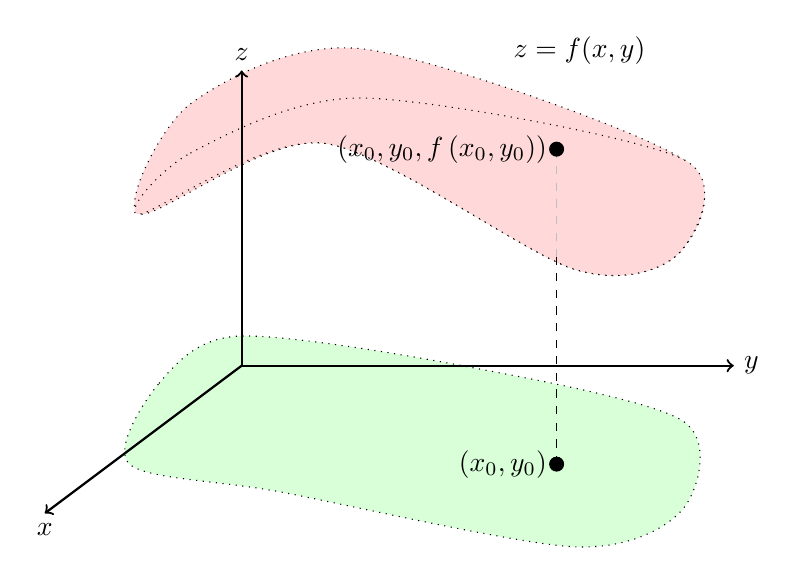
\begin{tikzpicture}[scale=1.25]
    \draw [dotted, fill=green!15] plot [smooth cycle] %
        coordinates {(-1.14,-1)(-0.84, -.18) (-0.04, 0.3) (2.24, 0) %
        (4.48, -0.56) (4.48, -1.46) (3.38,-1.84)(0.38, -1.28)};
    \draw [dotted, fill=red!15] plot [smooth cycle] %
        coordinates {(-1.04, 1.54) (-0.52, 2.66) (1.22, 3.22) %
        (4.48, 2.1)(4.44, 1.14) (3.38, 0.98) (0.84, 2.26)};
    %\shadedraw [color=red!15, inner color=red!5, outer color=red!15] (1,3) circle (2mm);
    \draw [dotted, fill=red!15] plot [smooth cycle] %
        coordinates {(-1.04, 1.54) (-0.52, 2.16) (1.22, 2.72) %
        (4.48, 2.1)(4.44, 1.14) (3.38, 0.98) (0.84, 2.26)};
    \draw[thick,->] (0,0) -- (-2,-1.5) node[below] {$x$};
    \draw[thick,->] (0,0) -- (5,0) node[right] {$y$};
    \draw[thick,->] (0,0) -- (0,3) node[above] {$z$};
    \filldraw (4.2,3.2) node[left] {$z=f(x,y)$};
    \draw [dashed] (3.2,-1) -- (3.2,1.1);
    \draw [dashed, lightgray] (3.2,1.1) -- (3.2,2.2);
    \filldraw (3.2,-1)circle (2pt) node[left] {$\left(x_0,y_0\right)$};
    \filldraw (3.2,2.2)circle (2pt) node[left] % 
        {$\left(x_0,y_0,f\left(x_0,y_0\right)\right)$};
\end{tikzpicture}
}

\end{frame}

% #########################################################################################
% #########################################################################################
% Slide 5 - Test3 - Curved shape of a surface
% #########################################################################################
% #########################################################################################

\section{Curved shape of a surface}
\begin{frame}
\frametitle{\textbf{Curved shape of a surface} }

Representing curved shape of a surface using PGF

\makebox[\textwidth][c]{ %
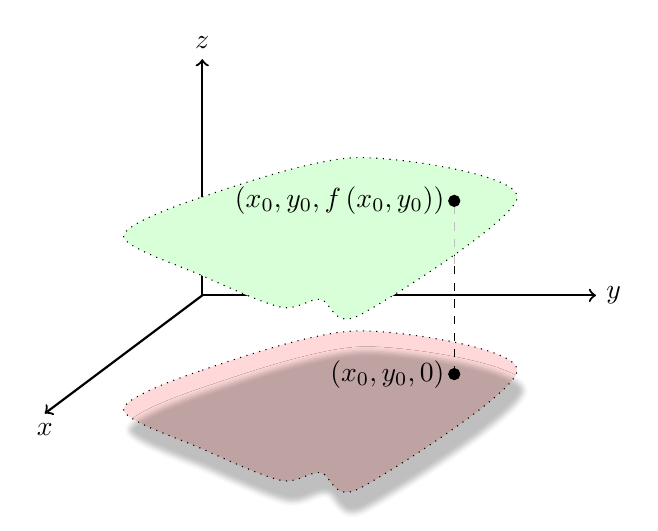
\begin{tikzpicture}[scale=1]
    \draw[thick,->] (0,0) -- (-2,-1.5) node[below] {$x$};% x axis
    \draw[thick,->] (0,0) -- (5,-0) node[right] {$y$};% y axis
    \draw[thick,->] (0,-0) -- (0,3) node[above] {$z$};% z axis
    
    \draw [dotted, fill=red!15]% red plain surface
    plot [smooth cycle]
    coordinates {(-1,-1.45) (0,-.95) (2,-.45) (4,-.95) (2,-2.45) (1.5,-2.25) (1,-2.35) %
    (0,-1.95)}; 
    
    \draw [dashed] (3.2,-1) -- (3.2,1.2);% segment
    
    \draw[dotted,fill=green!15,blur shadow={shadow yshift=-7em, shadow opacity=25}]% green surface
    plot [smooth cycle]
    coordinates {(-1,.75) (0,1.25) (2,1.75) (4,1.25) (2,-.25) (1.5,-.05) (1,-.15) (0,.25)};
    
    \draw [dashed, lightgray] (3.2,0.4) -- (3.2,1.2);% segment
    
    \filldraw (3.2,-1) circle (2pt)% point (x,y,0)
    node[left] {$\left(x_0,y_0,0\right)$};
    \filldraw (3.2,1.2) circle (2pt)% point (x,y,f)
    node[left] {$\left(x_0,y_0,f\left(x_0,y_0\right)\right)$};
    
\end{tikzpicture}
}

\end{frame}

% #########################################################################################
% #########################################################################################
% Slide 5 - Test3 - Curved shape of a surface
% #########################################################################################
% #########################################################################################

\section{Curved shape of a surface}
\begin{frame}
\frametitle{\textbf{Curved shape of a surface} }

Representing curved shape of a surface using PGF

\makebox[\textwidth][c]{ %
\begin{tikzpicture}
    \begin{axis}[view={-20}{20}, grid=both, xmin=0, ymin=0, zmin=0]

      \clip[
          rounded corners=5,
          x=1.1cm,y=.4cm,z=3cm,
          yshift=.1cm, xshift=-.7cm
      ]
          (.3,2) -- (0,1) -- (.5,.3) -- (1,.2) -- (2,1.3) -- (3.5,.5) --
          (4.5,2) -- (3.5,3) -- (1.5,3.4) -- (1.5,2.5) --
          cycle
          [yshift=2.7cm]
          (.3,2) -- (0,1) -- (.5,.3) -- (1,.2) -- (2,1.3) -- (3.5,.5) --
          (4.5,2)
          [rounded corners=0]
          parabola[parabola height=1.1cm] cycle
      ;

      \addplot3[surf] file {filename.txt};
      \addplot3[surf, point meta=explicit] table [z expr=0, meta index=2] {filename.txt};

    \end{axis}
\end{tikzpicture}
}

\end{frame}

\begin{filecontents*}{filename.txt}
    0 0 1.36
    1 0 1.50
    2 0 1.60
    3 0 1.69
    4 0 1.77
    5 0 1.80
    6 0 1.76
    7 0 1.68
    8 0 1.58
    9 0 1.41
    10 0 1.24
    
    0 1 1.46
    1 1 1.60
    2 1 1.73
    3 1 1.83
    4 1 1.92
    5 1 1.97
    6 1 1.95
    7 1 1.86
    8 1 1.73
    9 1 1.55
    10 1 1.37
    
    0 2 1.54
    1 2 1.69
    2 2 1.84
    3 2 1.97
    4 2 2.07
    5 2 2.12
    6 2 2.11
    7 2 2.02
    8 2 1.87
    9 2 1.68
    10 2 1.49
    
    0 3 1.56
    1 3 1.74
    2 3 1.92
    3 3 2.07
    4 3 2.18
    5 3 2.25
    6 3 2.24
    7 3 2.14
    8 3 1.99
    9 3 1.80
    10 3 1.59
    
    0 4 1.56
    1 4 1.74
    2 4 1.96
    3 4 2.13
    4 4 2.25
    5 4 2.32
    6 4 2.31
    7 4 2.22
    8 4 2.07
    9 4 1.86
    10 4 1.63
    
    0 5 1.56
    1 5 1.74
    2 5 1.95
    3 5 2.14
    4 5 2.27
    5 5 2.34
    6 5 2.33
    7 5 2.24
    8 5 2.09
    9 5 1.88
    10 5 1.64
    
    0 6 1.52
    1 6 1.71
    2 6 1.92
    3 6 2.09
    4 6 2.22
    5 6 2.29
    6 6 2.28
    7 6 2.20
    8 6 2.06
    9 6 1.87
    10 6 1.65
    
    0 7 1.45
    1 7 1.66
    2 7 1.85
    3 7 2.00
    4 7 2.11
    5 7 2.18
    6 7 2.18
    7 7 2.11
    8 7 1.98
    9 7 1.80
    10 7 1.61
    
    0 8 1.37
    1 8 1.56
    2 8 1.73
    3 8 1.87
    4 8 1.97
    5 8 2.04
    6 8 2.04
    7 8 1.98
    8 8 1.87
    9 8 1.71
    10 8 1.55
    
    0 9 1.29
    1 9 1.41
    2 9 1.57
    3 9 1.72
    4 9 1.82
    5 9 1.87
    6 9 1.87
    7 9 1.83
    8 9 1.74
    9 9 1.62
    10 9 1.47
    
    0 10 1.17
    1 10 1.25
    2 10 1.41
    3 10 1.55
    4 10 1.65
    5 10 1.70
    6 10 1.70
    7 10 1.66
    8 10 1.58
    9 10 1.48
    10 10 1.34
\end{filecontents*}
% #########################################################################################
% #########################################################################################
% Slide XX - Drawing ELBO reference image
% #########################################################################################
% #########################################################################################

\section{Drawing ELBO reference image}
\begin{frame}
\frametitle{\textbf{Drawing ELBO reference image}}
\centering
\begin{minipage}{1\textwidth}
    \centering
    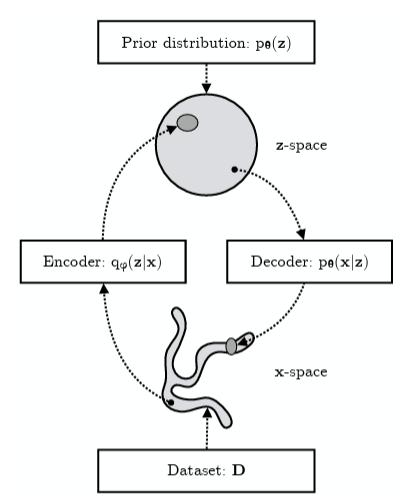
\includegraphics[width=0.5\textwidth]{images/ELBO-1.PNG} % Replace with your image file
    \captionof{figure}{ELBO reference image.}
\end{minipage}
\end{frame}

% #########################################################################################
% #########################################################################################
% Slide XX - Leatherback Observation Error reference image
% #########################################################################################
% #########################################################################################

\section{Leatherback Observation Error reference image}
\begin{frame}
\frametitle{\textbf{Leatherback Observation Error reference image}}
\centering
\begin{minipage}{1\textwidth}
    \centering
    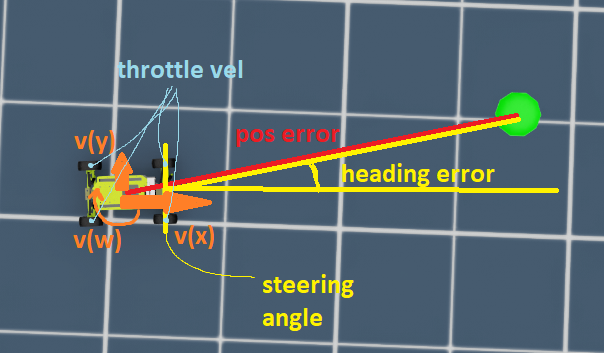
\includegraphics[width=0.8\textwidth]{images/observation_errors.png} % Replace with your image file
    \captionof{figure}{Leatherback Observation Error reference image.}
\end{minipage}
\end{frame}

% #########################################################################################
% #########################################################################################
% Slide XX - Conclusion
% #########################################################################################
% #########################################################################################

\section{Conclusion}
\begin{frame}
\frametitle{Conclusion}
The development of computer vision models has progressed rapidly, from YOLO’s fast and efficient real-time object detection to the powerful and flexible Vision Transformers. Both models represent milestones in the field, with YOLO excelling in speed and ViT pushing the boundaries of performance in image recognition. The future of computer vision is bright, with ongoing research promising even more breakthroughs.
\end{frame}

% #########################################################################################
% #########################################################################################
% #########################################################################################
% #########################################################################################

% ⠀⠀⠀⠀⠀⠀⠀⠀⠀⠀⠀⠀⠀⣀⣀⣀⡀⠀⠀⠀⠀⠀⠀⠀⠀⠀
% ⠀⠀⠀⠀⠀⠀⢀⣠⠤⠖⠈⠉⠉⠀⠀⠀⠀⠉⠢⡀⠀⠀⠀⠀⠀⠀
% ⠀⠀⠀⠀⠀⣴⠏⠀⠀⠀⠀⠀⠀⠀⠀⠀⠀⠀⠀⠈⢦⡀⠀⠀⠀⠀
% ⠀⠀⠀⣠⠞⠁⠀⠀⠀⠀⠀⠀⠀⠀⠀⢀⠞⠋⢙⣦⡈⣷⡄⠀⠀⠀
% ⠀⣀⠶⠁⠀⠀⣀⣀⡀⠀⠀⠀⠀⠀⡴⠁⠀⠀⠿⢿⡟⣌⢿⠀⠀⠀
% ⣠⡿⠀⢠⣜⠉⠀⠀⠙⢷⢄⠀⠀⠀⢧⠀⠀⠀⠀⠀⠀⠘⡆⢧⡀⠀
% ⣯⠃⠀⢾⣿⠗⠀⠀⠀⠀⡽⠀⠀⠀⠈⠳⢄⣀⠀⠀⠀⡰⠃⠘⣵⡄
% ⡏⠀⠀⠘⡄⠀⠀⠀⣠⠞⠁⠀⠀⠀⠀⠀⠀⠀⠉⠉⠁⠀⠀⠀⢱⡇
% ⡅⠀⠀⠀⠙⠒⠔⠚⠁⠀⠀⠀⠀⠀⠀⠀⠀⠀⠀⠀⠀⠀⠀⠀⠀⡇
% ⣧⡀⠀⠀⠀⠀⠀⠀⠀⠀⠀⠀⠀⠀⠀⠀⠀⢠⠀⠀⠀⠀⠀⠀⠀⡗
% ⡿⡇⠀⠀⠀⠀⠀⠀⠀⠀⠀⢠⡀⠀⠀⠀⠀⢸⡇⠀⠀⠀⠀⠀⠀⣇
% ⠹⣷⠀⠀⠀⠀⠀⠀⠀⠀⠀⠈⠷⣤⣤⣤⣤⠞⠁⠀⠀⠀⠀⠀⠀⣸
% ⠀⠸⣇⠀⠀⠀⠀⠀⠀⠀⠀⠀⠀⠀⠀⠀⠀⠀⠀⠀⠀⠀⠀⠀⣰⠇
% ⠀⠀⢇⠳⣄⠀⠀⠀⠀⠀⠀⠀⠀⠀⠀⠀⠀⠀⠀⠀⠀⠀⠀⢀⡏⠀
% ⠀⠀⠈⠀⠀⠉⠀⠀⠀⠀⠀⠀⠀⠀⠀⠀⠀⠀⠀⠀

% #########################################################################################
% #########################################################################################
% #########################################################################################
% #########################################################################################

\end{document}